\documentclass{article}

% Packages for code listing and syntax highlighting
\usepackage{listings}
\usepackage{xcolor}
\usepackage[margin=3cm]{geometry} % Adjust the margin value as desired
\usepackage{setspace}
\usepackage{tikz}
\usepackage{graphicx}
\usepackage{float}
\usepackage{textcomp}
\usepackage{multicol}
\usepackage{enumitem}

\onehalfspacing

% Define the color theme
\definecolor{codebackground}{RGB}{242, 242, 242}
\definecolor{codekeyword}{RGB}{0, 0, 255}
\definecolor{codecomment}{RGB}{63, 127, 95}
\definecolor{codestring}{RGB}{163, 21, 21}

% Code listing style for all languages
\lstdefinestyle{mystyle}{
    backgroundcolor=\color{codebackground},
    basicstyle=\footnotesize\ttfamily,
    keywordstyle=\color{codekeyword}\bfseries,
    commentstyle=\color{codecomment}\itshape,
    stringstyle=\color{codestring},
    numbers=left,
    numberstyle=\tiny\color{codecomment},
    stepnumber=1,
    numbersep=8pt,
    showstringspaces=false,
    breaklines=true,
    frame=single,
    frameround=none,
    framesep=5pt,
    rulecolor=\color{codebackground},
    tabsize=4,
    captionpos=b,
    xleftmargin=15pt,
    xrightmargin=15pt
}

% Set the default style for code listings
\lstset{style=mystyle}

% Additional packages and settings for math typesetting
\usepackage{amsmath}
\usepackage{amssymb}
\usepackage{bm}

% Define your document content
\begin{document}

\title{Functions Basics}
\author{Abyan Majid}
\date{\today}
\maketitle

\section{Definition}

\noindent A function in mathematics is some sort of relationship that can be established between two variables as input and output.

\vspace{\baselineskip}

\noindent Say that you have a variable $y$, of which value depends on another variable $x$. You write $y=f(x)$ to denote that "$y$ is a function of $x$" - and so $f(x)$ establishes that relationship that the value of $y$ depends on the value of $x$.

\section{Vertical line test - is that a function or not?}

To determine if a mathematical construct is a function, you can do the vertical line test - which states that if every vertical line $x=a$, where $a\in\mathbb{R}$, intersects the figure ONLY once, then this "figure" is a function. If it intersects more the once, it is not a function.

\begin{figure}[H]
    \centering
    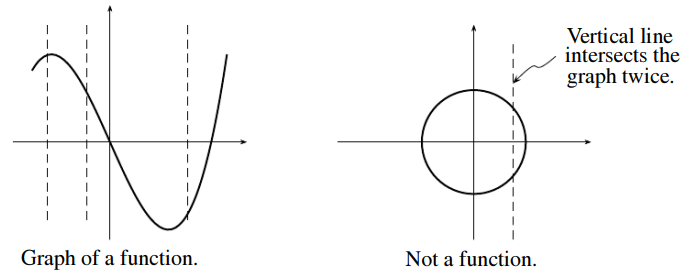
\includegraphics{../../../!assets/MATH1021-006-fig1.png}
    \caption{Vertical line test}
\end{figure}

\section{Domain and range}
\begin{itemize}
    \item A "\textbf{domain}" is the set of all possible INPUT values ($x$) for a function. To specify, the domain of a function $f(x)$, you write $\{x \phantom{1}| \phantom{1} x_1 \leq x \leq x_2 \}$, which is read as "all $x$ values, such that $x^1 \leq x \leq x_2$"
    \item A "\textbf{range}" is the set of all possible OUTPUT values ($y$) for a function. To specify the range of a function $f(x)$, you write $\{y \phantom{1}| \phantom{1} y_1 \leq y \leq y_2 \}$, which is read as "all $y$ values, such that $y_1 \leq y \leq y_2$"
    
\end{itemize}
Of course, you may replace the inequality sign with $<$, and you may also exclude one of the bounds. Or you may even say something like $x\in\mathbb{Z}$. It's all just set notation.

\section{Combining functions arithmetically}

If you have a function $f(x)$ and another $g(x)$, both of which have a common domain, you can combine the two by:
\begin{itemize}
    \item $f(x) + g(x)$
    \item $f(x) - g(x)$
    \item $f(x)\times g(x)$
    \item $f(x)\div g(x)$
\end{itemize}

\noindent Just combine respective terms as you would algebraically with any expression.

\section{Composite function}
A "composite function", denoted as $(f \circ g)(x)$ or $f(g(x))$, is essentially a function that takes another function as an input.

\begin{center}
    So if we have $f(x)=2x^2+4x-1$ and $g(x)=2x+5$, our composite function would be:
    $$(f\circ g)=f(g(x))=2(2x+5)^2+4(2x+5)-1$$
    You can choose to simplify it further, like so:
    $$=8x^2+48x+69$$
\end{center}

\section{Inverse function}
The "inverse" of the function $f(x)$, denoted as $f^{-1}(x)$, is the reflection of $f(x)$ about the line $y=x$ in the cartesian plane. To find the inverse of a function, you do as demonstrated in the following example:

\begin{center}
    Find the inverse of the function $f(x)=-\frac{1}{3}x+1$
\end{center}

\begin{enumerate}
    \item Rewrite $f(x)$ as $y$ or any other variable besides the input.
    $$y=-\frac{1}{3}x+1$$
    \item Switch $y$ and $x$.
    $$x=-\frac{1}{3}y+1$$
    \item Solve for $y$.
    $$x=-\frac{1}{3}y+1$$
    $$3x=-y+3$$
    $$3x-3=-y$$
    $$y=-3x+3$$
    \item $y$ is now the inverse of $f(x)$, therefore rewrite $y$ as $f^{-1}(x)$.
    $$f^{-1}(x)=-3x+3$$
\end{enumerate}

\end{document}